\documentclass[a4paper,12pt,oneside,openany,table,xcdraw]{article}

\usepackage{setspace}
\usepackage{multirow}
\usepackage{hyperref}
\usepackage{caption}
\usepackage{indentfirst}

\usepackage[brazilian]{babel}
\usepackage[utf8x]{inputenc}
\usepackage{amsmath, graphicx, mathptmx, enumerate}
\usepackage{float, verbatim}
\usepackage[colorinlistoftodos]{todonotes}
\usepackage{makeidx} % Para o sumário
\usepackage{geometry}
\usepackage{multicol}
\usepackage{subfigure}

\graphicspath{{../img/}}
\geometry{a4paper, hmargin={3cm, 3cm}, vmargin={3cm, 2cm} }
\setlength{\parindent}{1.0cm}
\captionsetup{font=small}

\begin{document}
\newcommand{\thedepartment}{Faculdade de Engenharia Elétrica}
\newcommand{\thecourse}{FEELT}
\newcommand{\thetitle}{AMPLIFICADOR DIFERENCIAL}
\newcommand{\thetype}{Relatório da Disciplina de Eletrônica Analógica II}
\newcommand{\theproftitle}{Bacharel em Engenharia Elétrica}
\newcommand{\thestudent}{Lesly Viviane Montúfar Berrios\\
\centering11811ETE001}
\newcommand{\theadvisor}{Prof. Gustavo Brito de Lima}
\newcommand{\thecity}{Uberlândia}

\thispagestyle{empty}\newcommand*{\themonth}{\ifthenelse{\the\month < 2}{Janeiro }
                  {\ifthenelse{\the\month < 3}{Fevereiro }
                  {\ifthenelse{\the\month < 4}{Março }
                  {\ifthenelse{\the\month < 5}{Abril }
                  {\ifthenelse{\the\month < 6}{Maio }
                  {\ifthenelse{\the\month < 7}{Junho }
                  {\ifthenelse{\the\month < 8}{Julho }
                  {\ifthenelse{\the\month < 9}{Agosto }
                  {\ifthenelse{\the\month < 10}{Setembro }
                  {\ifthenelse{\the\month < 11}{Outubro }
                  {\ifthenelse{\the\month < 12}{Novembro }{Dezembro }}}}}}}}}}}}
                  
\begin{titlepage}
\begin{center}

	\vspace{-0.5cm}

  \begin{figure}[hbt!]
		\begin{center}
		   
\includegraphics[width=2.8cm]{ufu-logo.png}
		\end{center}
	\end{figure}
 	%\vspace{-4cm}

%\begin{doublespacing}

  \Large{\textbf{Universidade Federal de Uberlândia}}\\
  \large{\thedepartment}\\
  \large{\thecourse}\\


\vspace{5.8cm}
  \par
  \large\textbf{\thetitle}
\vspace{5.8cm} 

%\end{doublespacing}
  \par
  \thetype\\
  por\\
  %\hspace{2cm}\large{}\\

\vspace{0.8cm}
\par
  \normalsize{\thestudent}\\ [2cm]
  \theadvisor

\par\vfill
  \thecity, \themonth / \the\year

\end{center}

\end{titlepage}

%% Comeca o documento !

\onehalfspacing
\tableofcontents % sumário
\newpage

 %%%%%%%%%%%%%%%%%%%%%%%%%%%%%%%%%%%%%%%%%%%%%%%%%%%%%%%%%%%%%%%%%%%%%%%%%%%%
\section{Objetivos} % 2,5 %


 %%%%%%%%%%%%%%%%%%%%%%%%%%%%%%%%%%%%%%%%%%%%%%%%%%%%%%%%%%%%%%%%%%%%%%%%%%%%
\section{Introdução teórica} 
%qu'Est-ce que c'est? Histoire


% À quoi ça sert? Applications
O amplificador diferencial é o estágio de entrada da maioria dos amplificadores operacionais, daí a importância de estudá-lo. Além disso, tem a função de aumentar a impedância de entrada, reduzir a corrente de polarização e o offset da tensão de saída. A Figura \ref{intro:amp-dif} exemplifica a estrutura de um amplificador diferencial.

\vspace{0.5cm}
\begin{figure}[H]
\centering
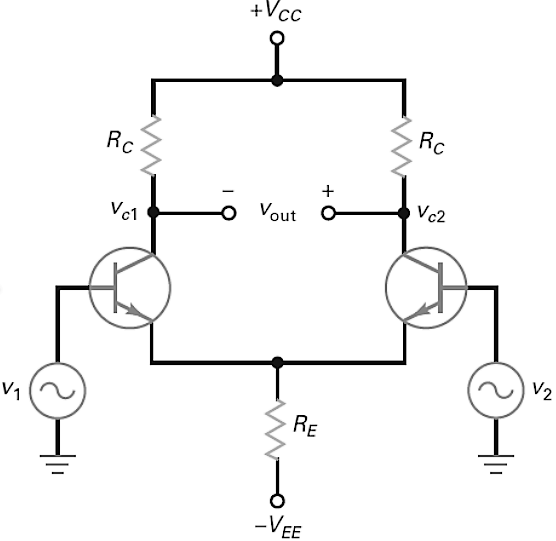
\includegraphics[width=13cm]{amp-dif}
\caption{Amplificador diferencial.}
\label{intro:amp-dif}
\end{figure}
\vspace{0.5cm}

Nesse circuito, a relação entre entrada e saída é dada como na Equação \ref{vout}, e, da análise em conrente contínua (CC), percebe-se que o offset de tensão de saída é nulo quando as tensões de entrada estão em fase e são de mesma amplitude.

\begin{equation} \label{vout}
V_{out} = A_v\ (V_{in} ^+ - V_{in} ^-)
\end{equation}


 %%%%%%%%%%%%%%%%%%%%%%%%%%%%%%%%%%%%%%%%%%%%%%%%%%%%%%%%%%%%%%%%%%%%%%%%%%%%
\section{Procedimento Experimental}
\subsection{Materiais e ferramentas} % 2,5%

\singlespacing
\begin{itemize}
\begin{multicols}{2}
\item \emph{2 transistores BC337 ou similar;}
\item \emph{2 resistores 6k8;}
\item \emph{1 resistor 5k6;}
\item \emph{1 resistor de 1k;}
\item \emph{1 resistor de 100k;}\columnbreak

\item \emph{1 Fonte de alimentação simétrica;}
\item \emph{1 Multímetro;}
\item \emph{1 Gerador de Funções;}
\item \emph{1 Osciloscópio}
\end{multicols}

\end{itemize}
\onehalfspacing

\vspace{0.2cm}
\subsection{Montagem} % 2,5%
A montagem a ser utilizada no experimento trata-se do amplificador diferencial da Figura \ref{proc:montagem}, o qual será analisado a nível CC e CA.

\vspace{0.5cm}
\begin{figure}[H]
\centering
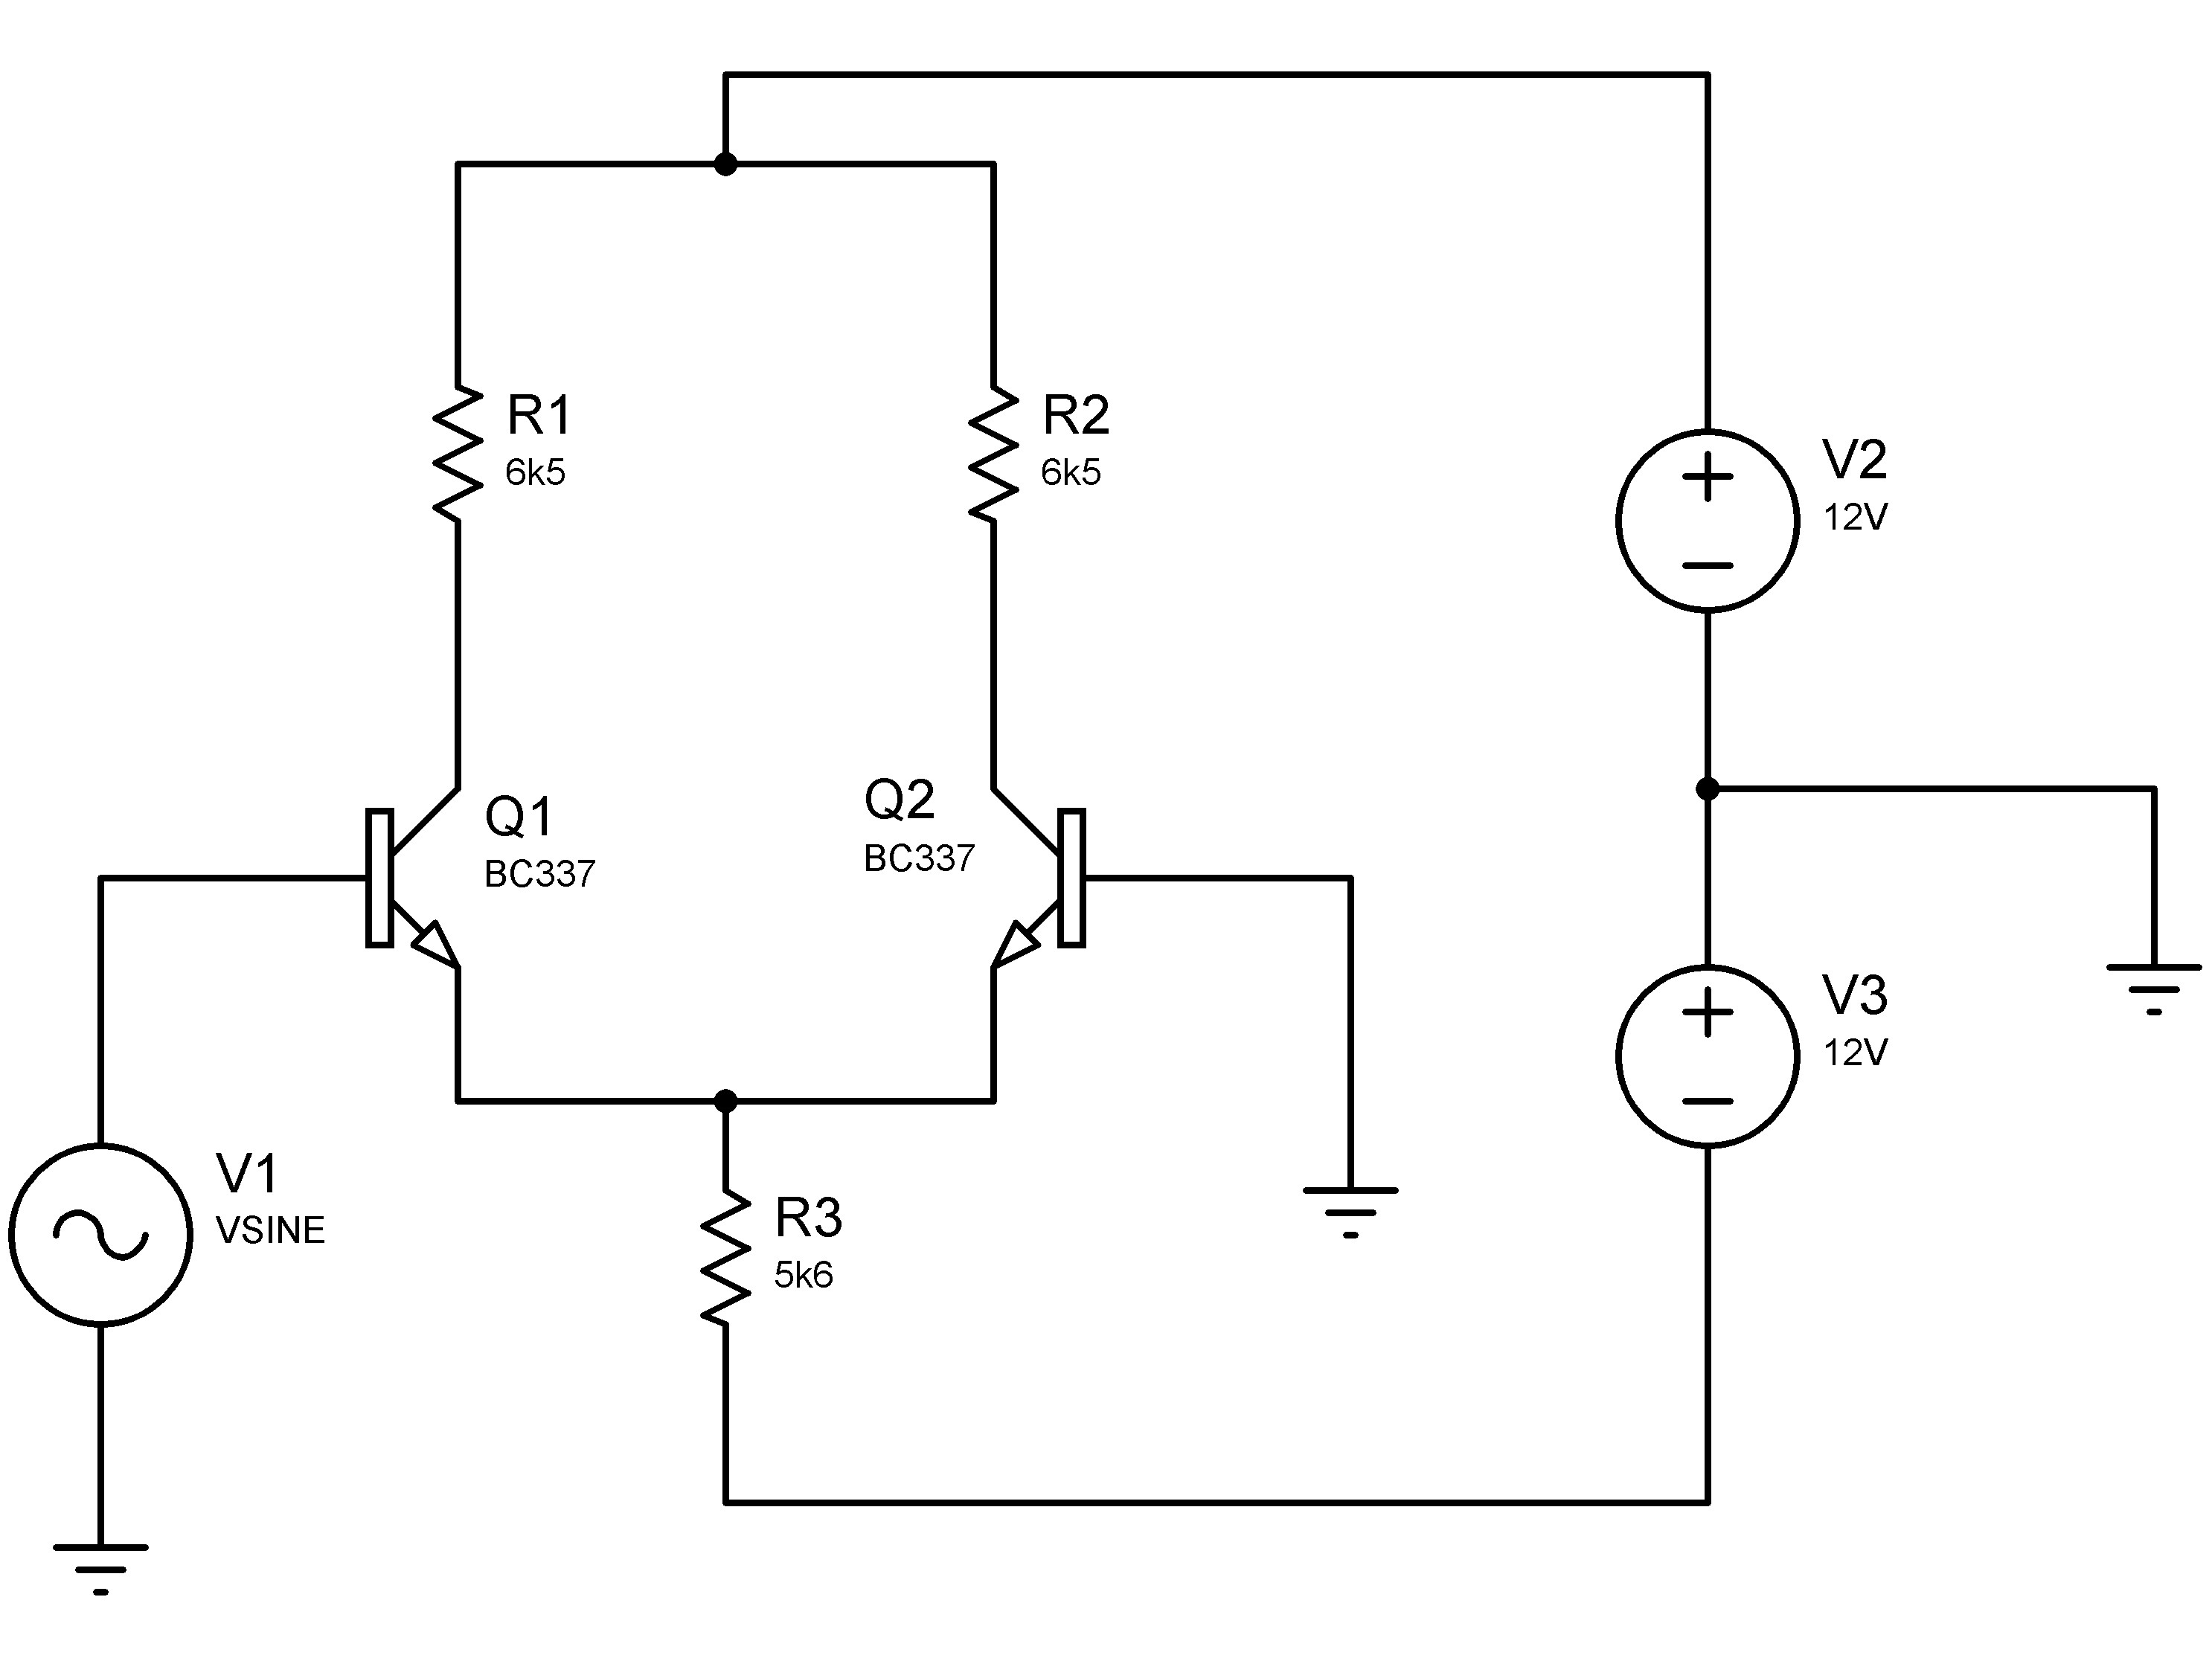
\includegraphics[width=13cm]{montagem}
\caption{Montagem do amplificador diferencial.}
\label{proc:montagem}
\end{figure}
\vspace{0.5cm}

Assim, da análise a nível CC tem-se o circuito da Figura \ref{proc:CC}, enquanto que para o nível CA, o da Figura \ref{proc:CA}.

 \vspace{0.5cm}
\begin{figure}[H]
\center
\subfigure[][]{\label{proc:CC}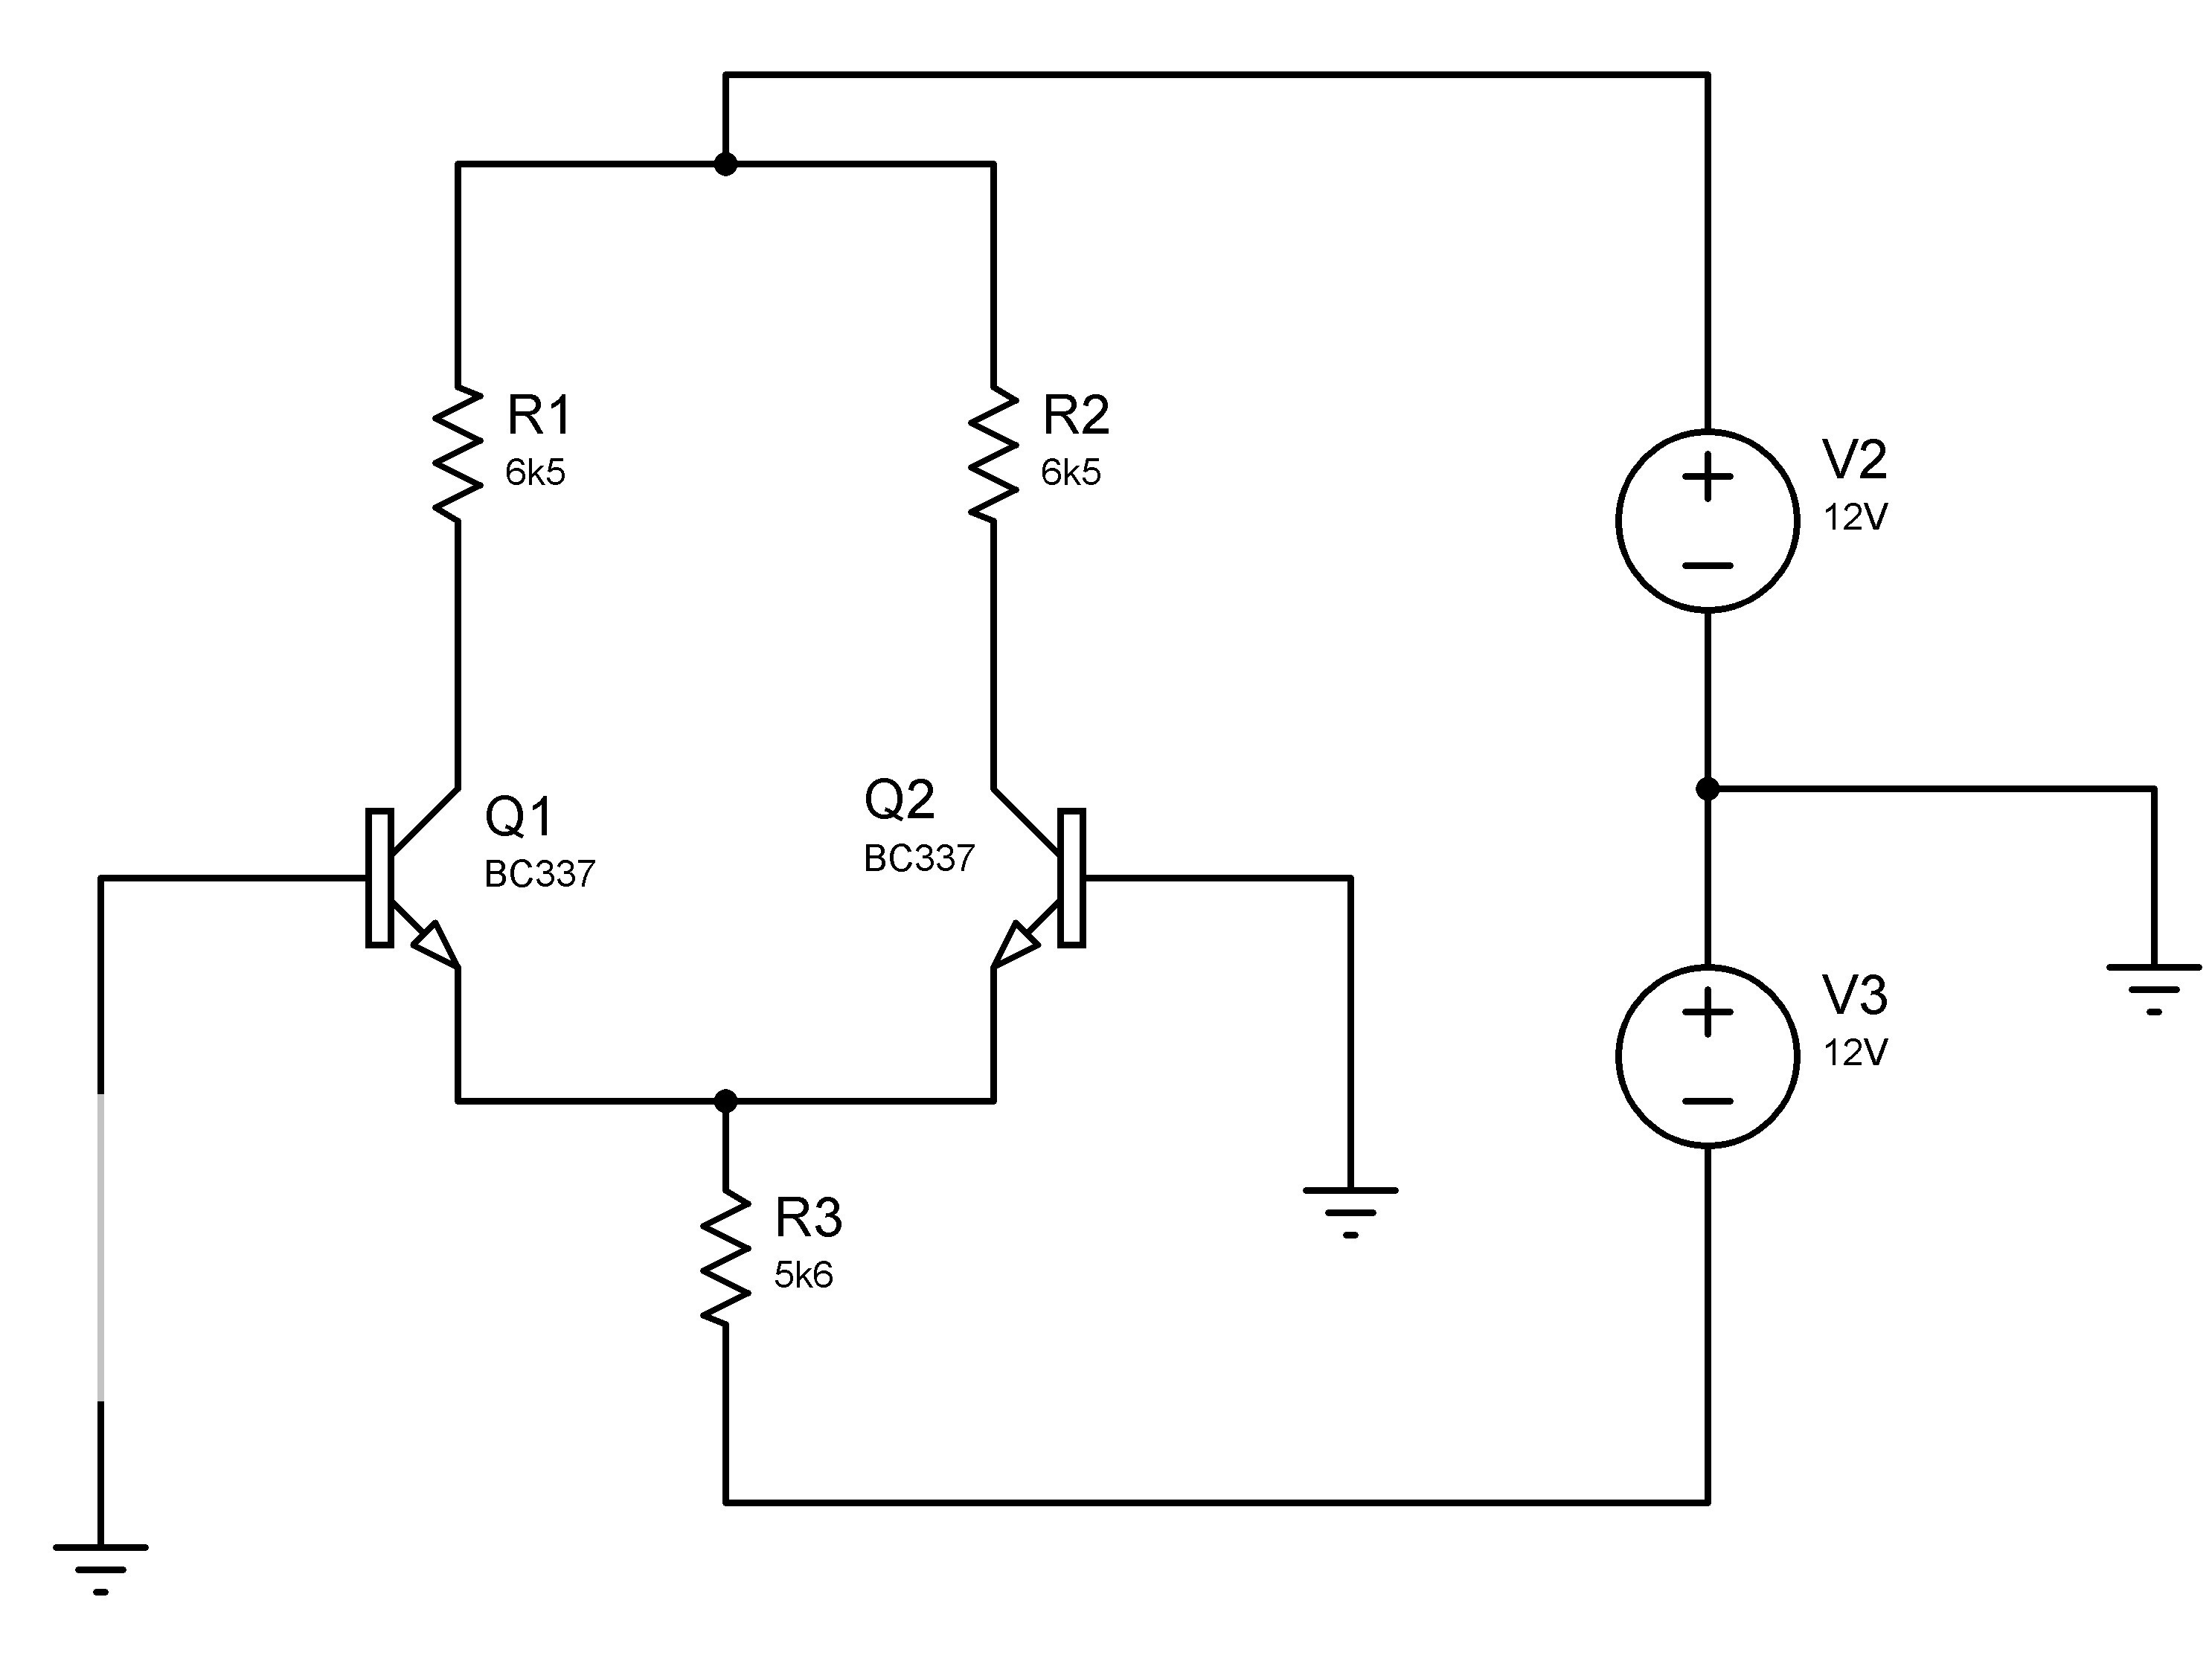
\includegraphics[height=5cm]{CC}}
\qquad
\subfigure[][]{\label{proc:CA}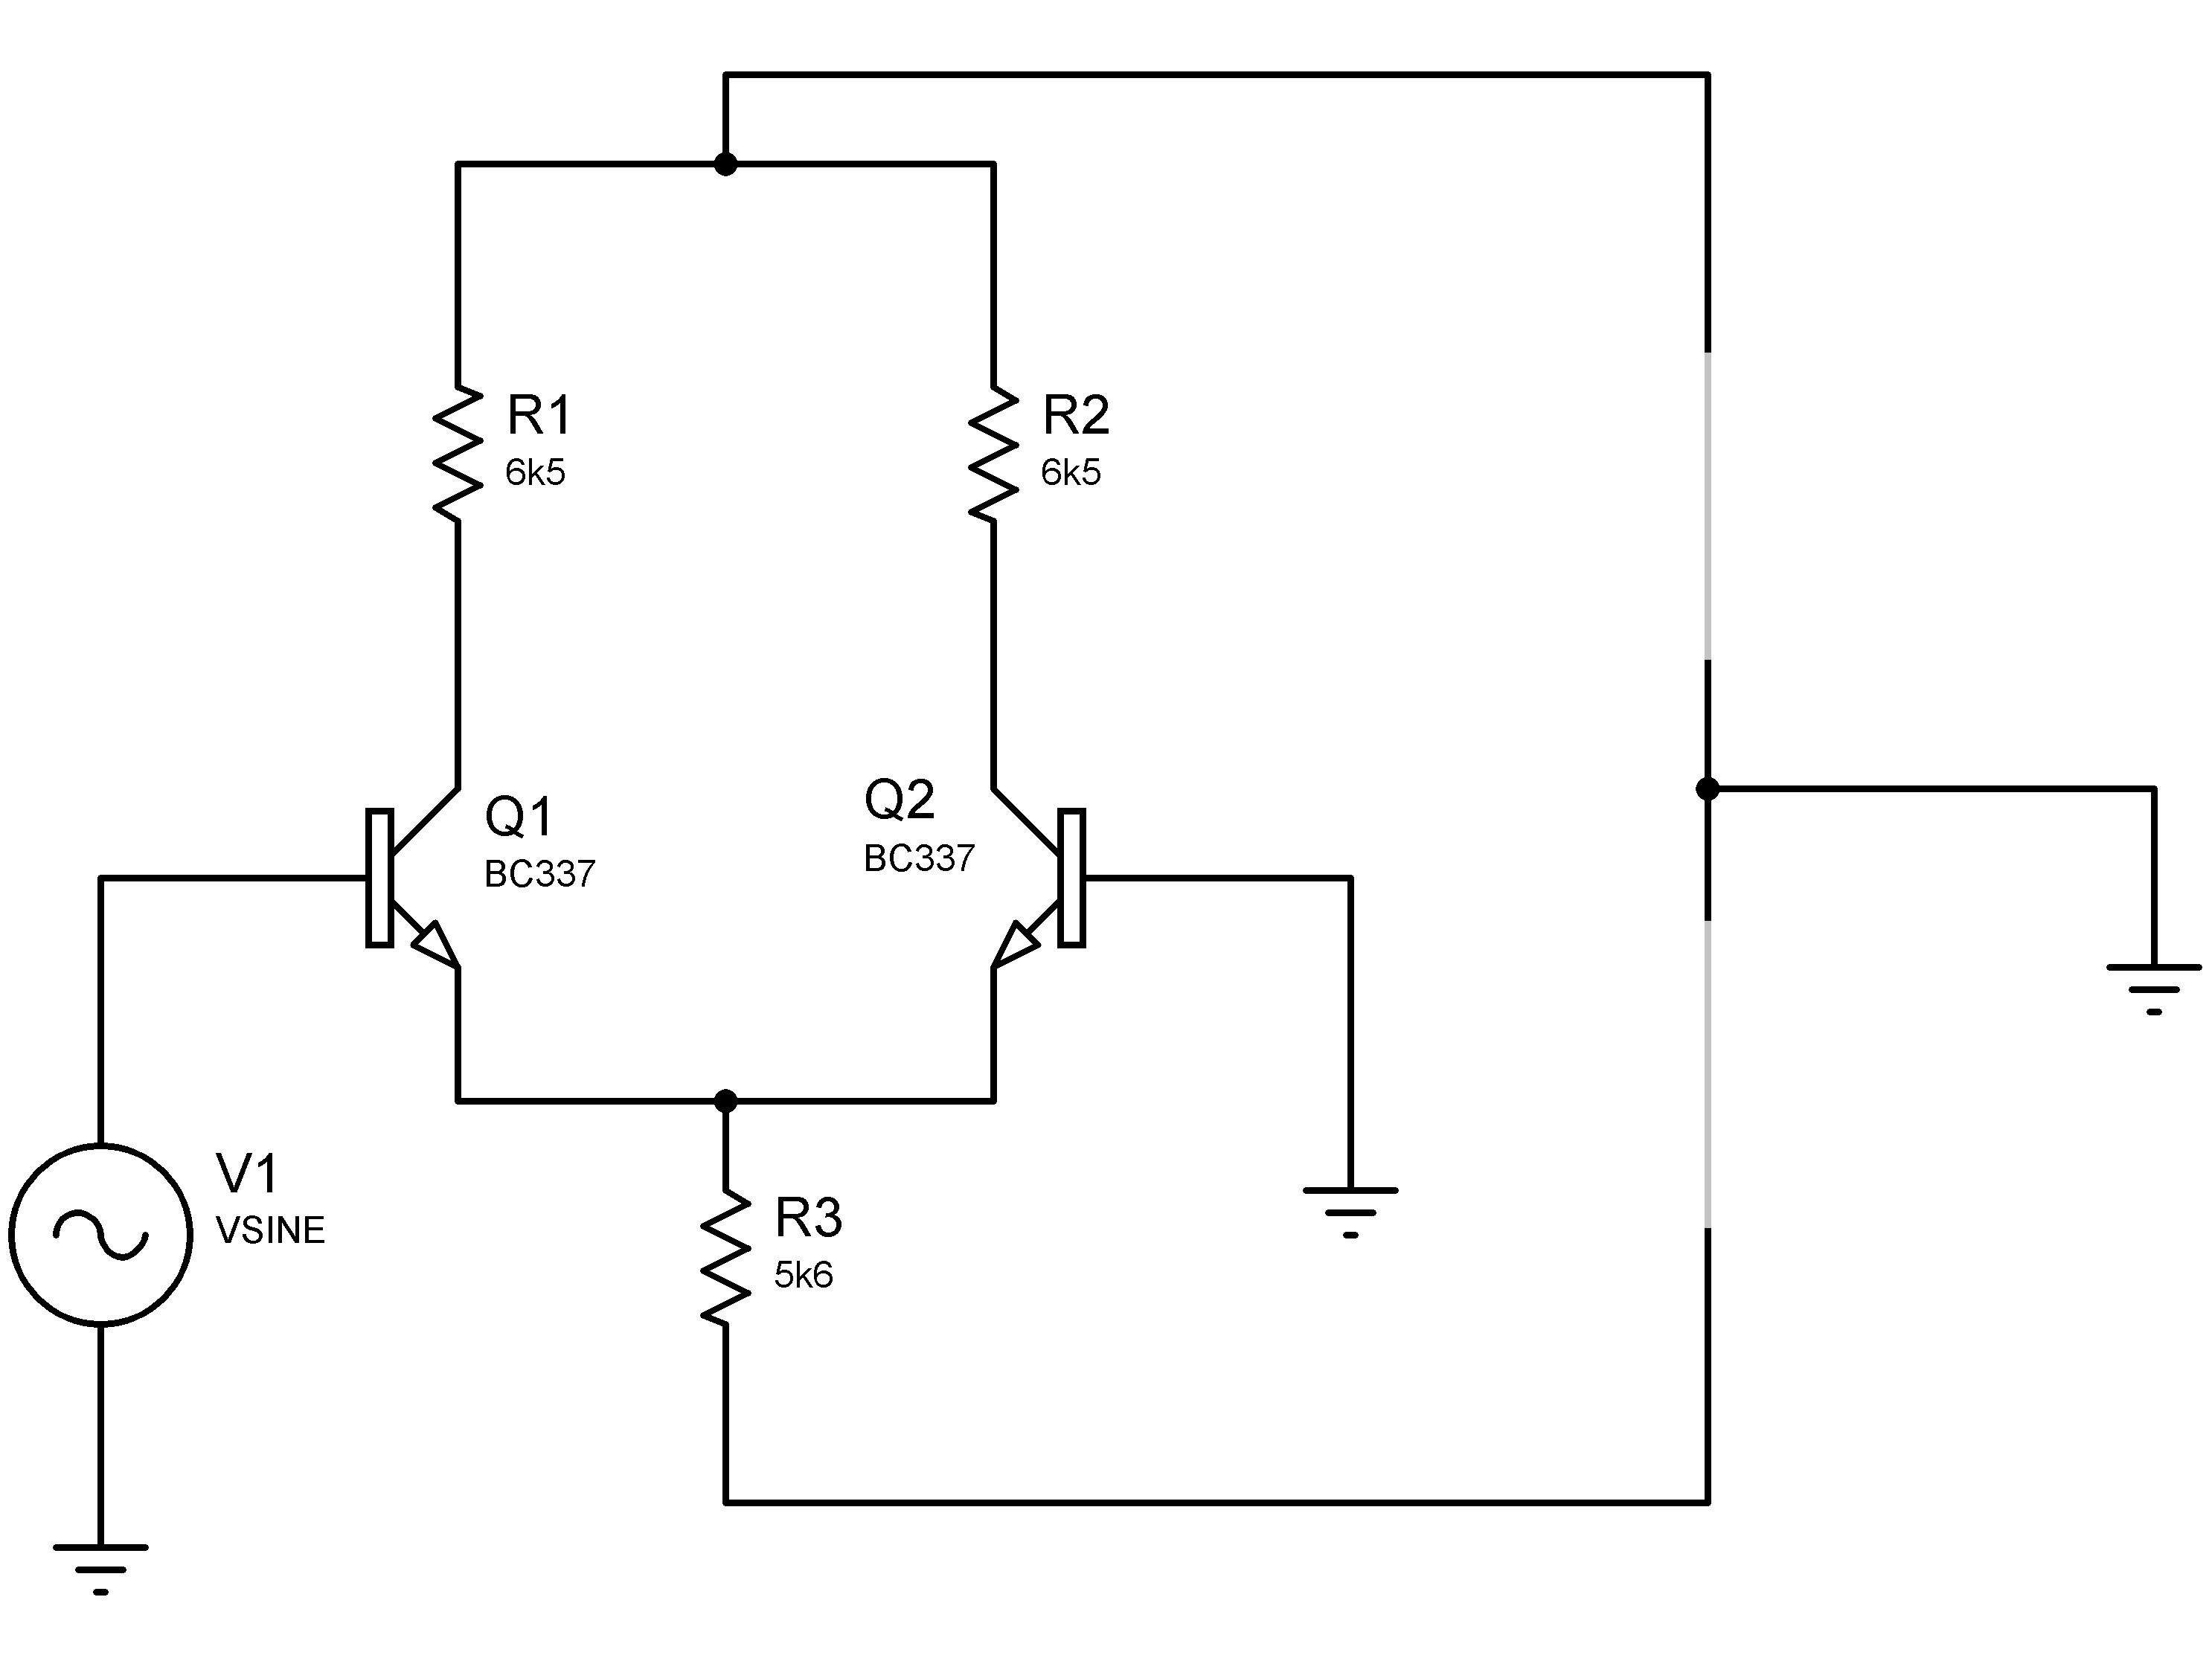
\includegraphics[height=5cm]{CA}}
\caption{Análise (a) CC e (b) CA do circuito amplificador diferencial.}
\label{proc:analise}
\end{figure}
\vspace{0.5cm}

 %%%%%%%%%%%%%%%%%%%%%%%%%%%%%%%%%%%%%%%%%%%%%%%%%%%%%%%%%%%%%%%%%%%%%%%%%%%%
\section{Simulação} %(10%);
Da simulação computacional, pode-se confirmar os valores das grandezas teóricas. Utilizando-se o software \emph{PROTEUS}, a simulação do esquemático da Figura \ref{sim:circuito} fornece os dados dispostos na Tabela \ref{sim:dados}.

 \vspace{0.5cm}
\begin{figure}[H]
\centering
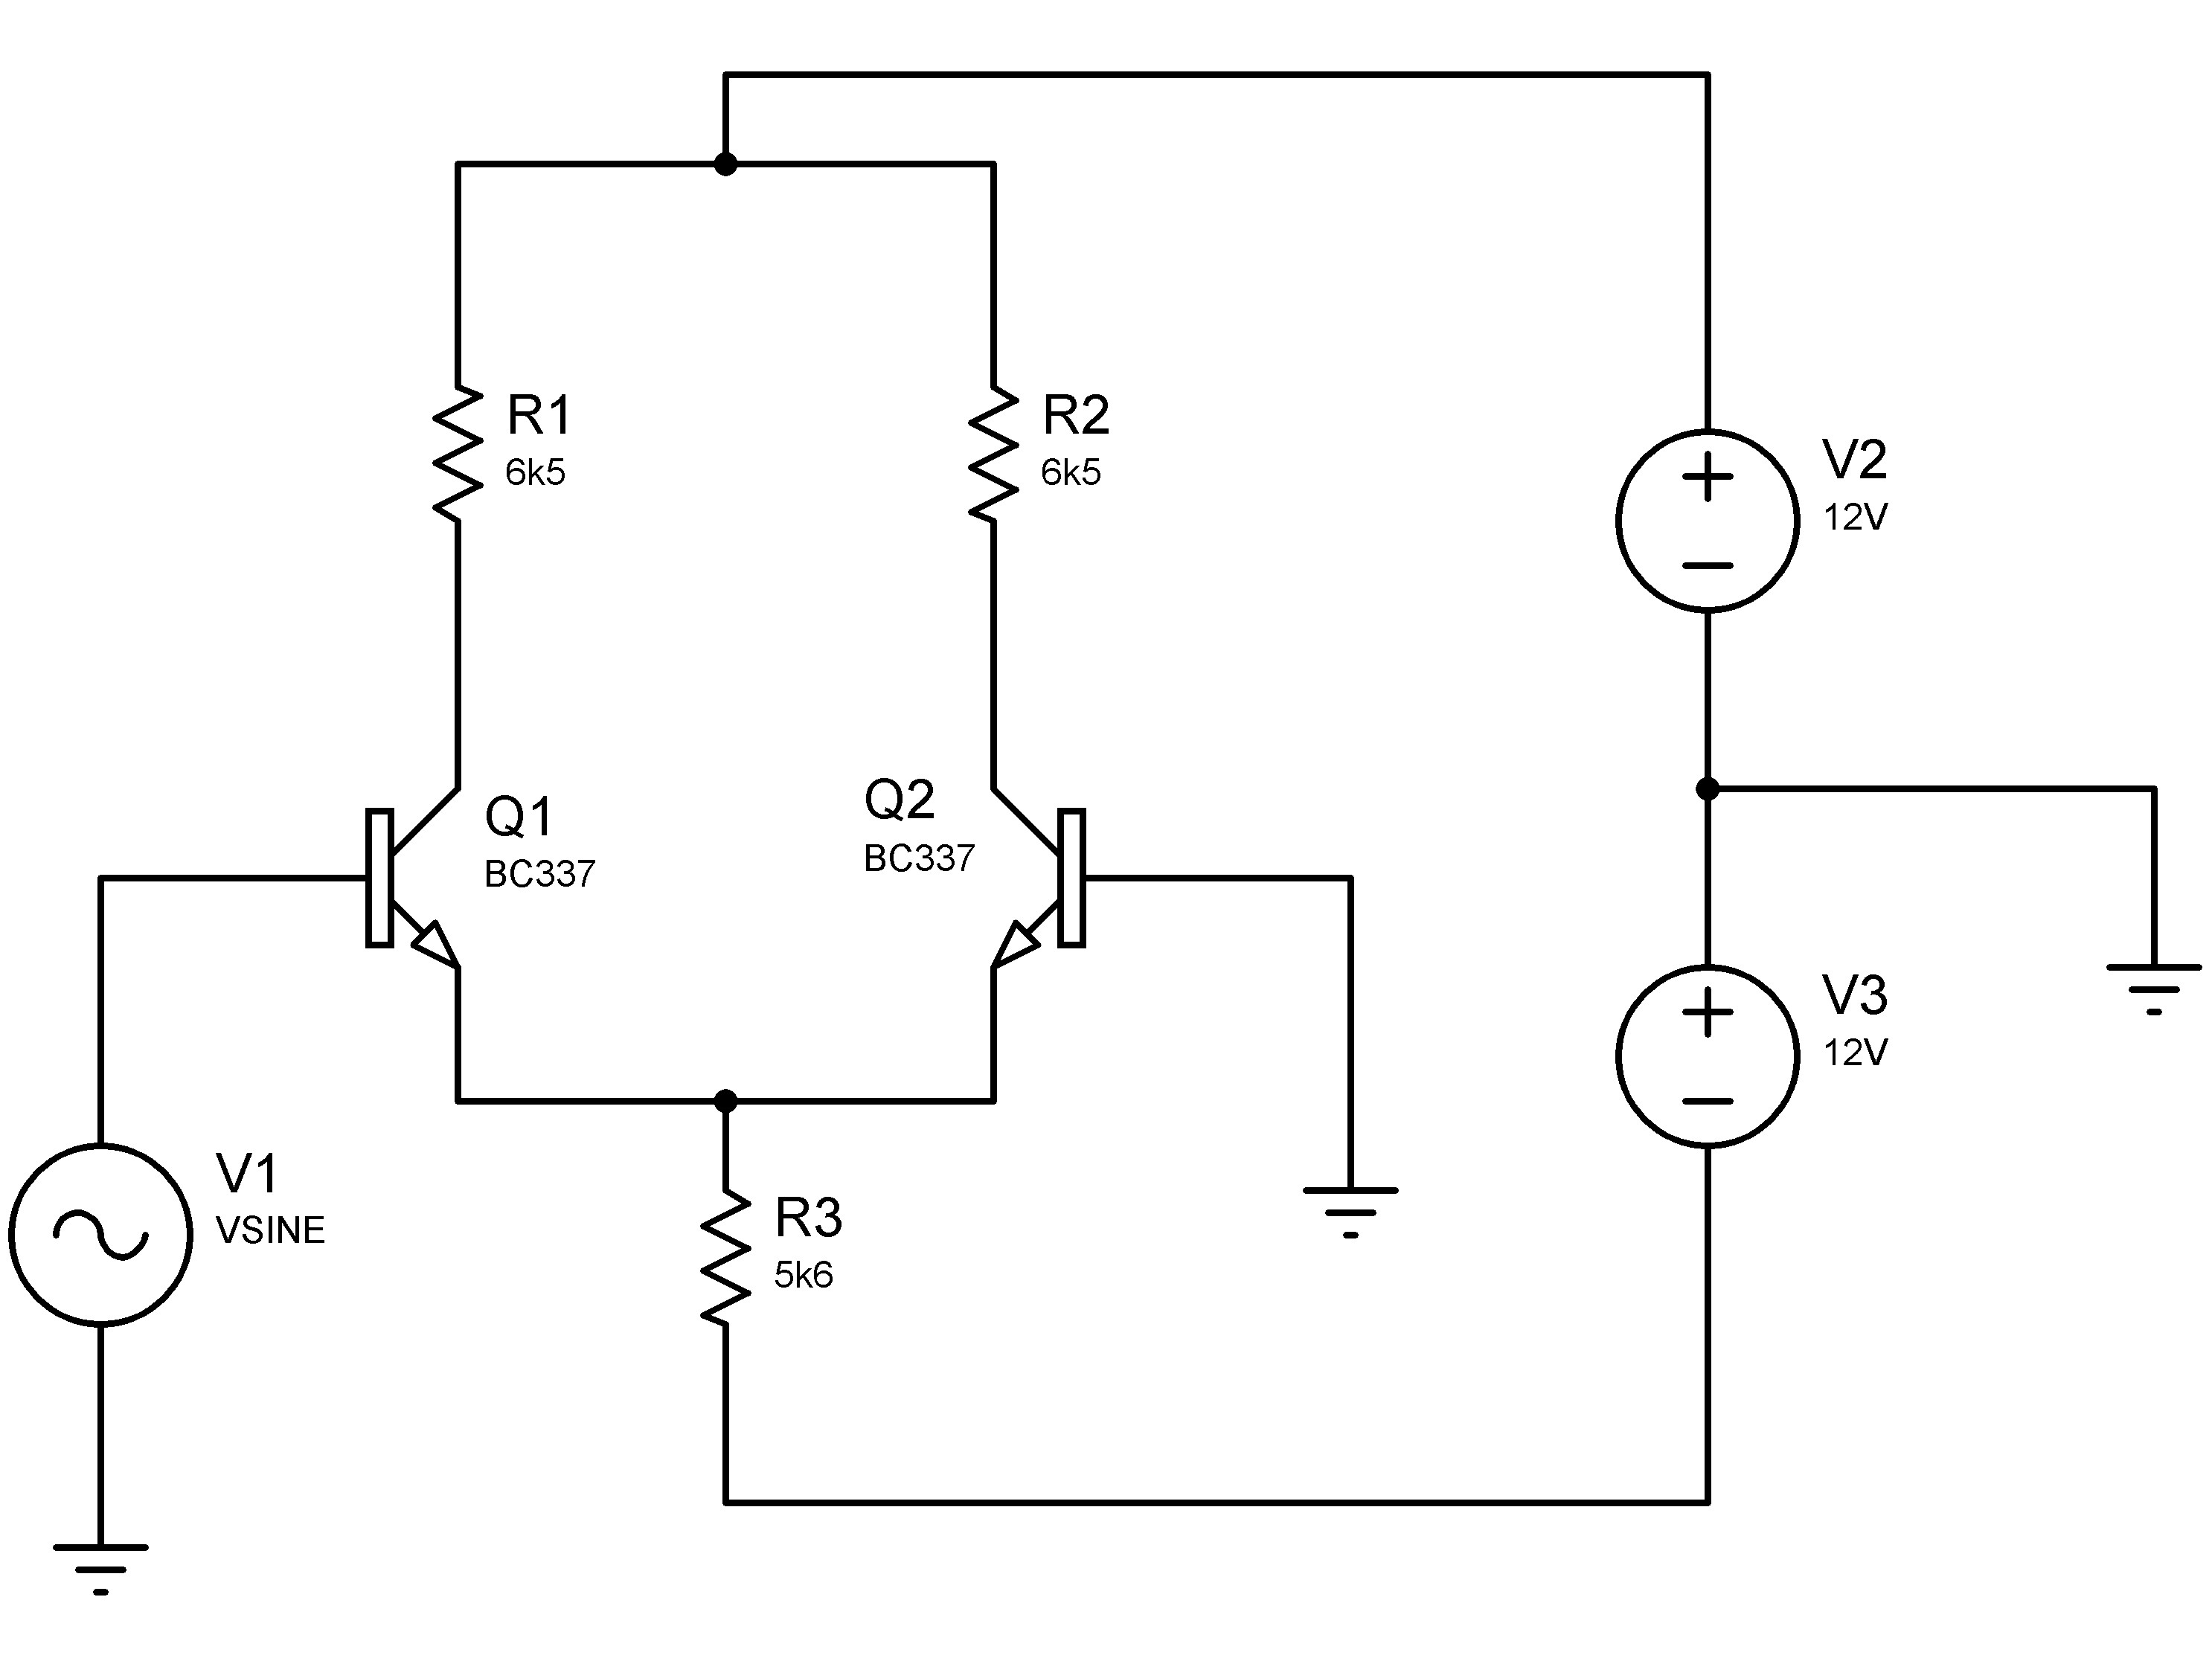
\includegraphics[width=13cm]{sim-circuito}
\caption{Circuito esquemático.}
\label{sim:circuito}
\end{figure}
\vspace{0.5cm}

% tabela

 %%%%%%%%%%%%%%%%%%%%%%%%%%%%%%%%%%%%%%%%%%%%%%%%%%%%%%%%%%%%%%%%%%%%%%%%%%%%
\section{Resultados e Discusões} %(quando houver) (70%)
Primeiramente, na Tabela \ref{dis:comp}, tem-se a comparação entre os dados teóricos, experimentais e de simulação, dos quais não se espera grande diferença, à exceção dos experimentais, que podem sofrer alteração de condições devido ao meio - que gera incerteza na medida.

% tabela

 %%%%%%%%%%%%%%%%%%%%%%%%%%%%%%%%%%%%%%%%%%%%%%%%%%%%%%%%%%%%%%%%%%%%%%%%%%%%
\section{Conclusões} % (no mínimo 10 linhas) (5%)

\newpage
\begin{thebibliography}{9} 
% Introdução
\bibitem{sedra}
    Sedra, A.; Simth, K; 
    “Análise de Circuitos Em Engenharia”, Oxford University Press, $5^a$ Ed., 2004.

\bibitem{malvino}
    Malvino; 
    “Eletrônica”, Pearson, $5^a$ Ed., 2004.

\bibitem{boylestad}
    Boylestad, R;
    “Intrdução À Análise de Circuitos”, Pearson, $10^a$ Ed., 2004.

\end{thebibliography}
\end{document}
